% Created 2025-03-29 Sat 12:43
% Intended LaTeX compiler: lualatex
\documentclass[11pt]{article}
\usepackage{fontspec}
\usepackage{graphicx}
\usepackage{lilyglyphs}
\usepackage{graphicx}
\usepackage{longtable}
\usepackage{wrapfig}
\usepackage{rotating}
\usepackage[normalem]{ulem}
\usepackage{amsmath}
\usepackage{amssymb}
\usepackage{capt-of}
\usepackage{hyperref}
\usepackage[cm]{fullpage}
\usepackage[headheight=15pt, headsep=10pt, top=1in, bottom=1in, left=0.75in, right=0.75in]{geometry} % Ensure sufficient header space
\usepackage{fancyhdr}
\pagestyle{fancy}
\fancyhf{}
\fancyhead[L]{\textbf{ii-V-I Snippets}} % Left header with title
\fancyhead[R]{\textbf{Bartev - Lesson 27 (2025-03)}} % Right header with author
\fancyfoot[C]{\thepage}
\fancyfoot[R]{Printed \today} % Right footer with today's date
\renewcommand{\headrulewidth}{0.4pt} % Optional: Add a horizontal rule below the header
\makeatletter
\let\ps@plain\ps@fancy % Apply "fancy" style to the first page
\let\maketitle\relax % Suppress default title/author rendering
\makeatother
\author{Bartev}
\date{\today}
\title{Sax Lesson 27}
\hypersetup{
 pdfauthor={Bartev},
 pdftitle={Sax Lesson 27},
 pdfkeywords={},
 pdfsubject={},
 pdfcreator={Emacs 29.4 (Org mode 9.6.15)}, 
 pdflang={English}}
\begin{document}

\maketitle
\tableofcontents


\section{Assignment}
\label{sec:org02bc423}

Hey Bartev,

As per usual, awesome work on everything in your last assignment! Here are some ideas for your 27th assignment:

\subsection{Solo Transcription}
\label{sec:orgd719371}
Joe Henderson on Song for my Father - This is an iconic solo and record and one of my favorite things about this solo is Joe's use of motivic development and rhythm. He's so great at maintaining interest and developing ideas throughout his entire solo. Let's transcribe as much as we can on this and then try to ALSO solo over this tune in a similar manner.

\href{https://www.youtube.com/watch?v=CWeXOm49kE0}{Song For My Father (youtube)}

\subsection{Technique}
\label{sec:orgcfe0885}
Now that we worked on the intervals in our major scales, let's do the same thing for melodic minor and harmonic minor. We can also alternate the direction, so for example, instead of playing C E D F E G and so forth, we can work these by playing the first interval ascending and the second descending: C E F D E G A F\ldots{}. try working like this now to change things up as you get into melodic and harmonic minor.


\subsection{Tune}
\label{sec:orgdaf4d02}
Let's learn the melody to Nica's Dream by Horace Silver and work on improvising through this tune in the original key.

\subsection{Composition}
\label{sec:org17f5176}
Let's compose 10 ii V lines that specifically use minor major 7 on the ii-7 and half whole diminished on the V7. Feel free to resolve these to major OR minor resolution chords!

\section{Technique}
\label{sec:orgb4c416f}
Melodic (\flat3) and harmonic (\flat3, \flat6) minor scales
\section{Variations on chord changes}
\label{sec:orga94e8d1}

\subsection{Major ii-V-I}
\label{sec:org98d0689}
\begin{center}
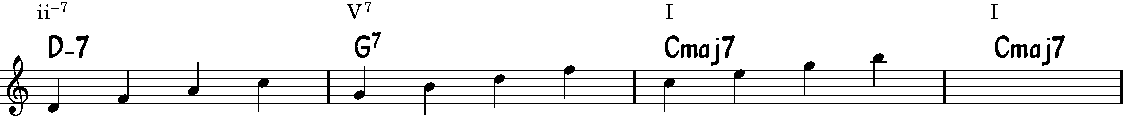
\includegraphics[width=.98\linewidth]{major_ii_v_i.pdf}
\end{center}

\section{Understanding the chords in Nica’s Dream}
\label{sec:org7f07a11}

\subsection{A section}
\label{sec:org0c12c49}

BV: m12 there’s a D7\#9\#5 into G7\#5

2 chords with almost no notes in common.

What is this progression, and what do you play over these chords?


dom7\sharp5 is just another way to say dom7alt or dom7\sharp9 (dominant diminished).

So, your options:

D7\sharp5\sharp9
\begin{itemize}
\item D altered (Eb melodic minor)
\item D H/W diminished (D, E\flat,  F, F\sharp,  G\sharp,  A, B, C)
\end{itemize}

G7\sharp5
\begin{itemize}
\item G altered (A\flat   melodic minor)
\item G H/W diminished (G, A, B\flat, C, C\sharp, D\sharp, E, F\sharp)
\end{itemize}

\subsection{B section}
\label{sec:org44afbcf}

dom7sus is the same as mixolydian but with more emphasis on the 4th, rather than the third! A nice shortcut you could also use is major pentatonic from the b7. So,

B\flat 7sus
\begin{itemize}
\item Bb mixolydian
\item Ab major pentatonic
\end{itemize}

BV: I see the G half dim and I want to think minor ii-V, but the V has a \#5, and it’s resolving to a dominant, not minor

You are indeed to think of that as a minor ii-V! The C7\#5 is the same thing as a C7b13. It's sort of an "incomplete" chord, offering you the freedom to chose C7b9b13, C7alt, or C7\#5\#9 (dominant diminished). All of the options will sound great. Just pick your most comfortable for now and stick with that one!

BV: Then the F\#-7 B7 goes into a Bb7sus. What is this?

B7 to Bb7sus is a tritone substitution approach! F7 to Bb7 is what it's swapping with.
\end{document}
